\documentclass{article}[12pt]
\usepackage[section]{placeins}
\usepackage[utf8]{inputenc}
\usepackage{graphicx}
\usepackage[a4paper,width=150mm,top=25mm,bottom=25mm,bindingoffset=6mm]{geometry}
\usepackage{amsmath,amssymb}
\usepackage{subfig}
\usepackage{setspace}
\usepackage[toc,page]{appendix}

\usepackage{caption}

\usepackage{listings}
\lstset{language=R,
    basicstyle=\small\ttfamily,
    morekeywords={TRUE,FALSE},
    deletekeywords={data,frame,length,as,character},
    keywordstyle=\color{blue},
}

\usepackage{ntheorem} % For writing hypotheses
\theoremseparator{:} % Insert :

\newtheorem*{hyp*}{Hypothesis \protect\hypnumber} % Name "Hypothesis"
\newenvironment{hyp}[1]{\renewcommand{\hypnumber}{#1}\begin{hyp*}}{\end{hyp*}}
\newcommand{\hypnumber}{}

\usepackage{xcolor}
\usepackage{xparse}
\NewDocumentCommand{\codeword}{v}{%
\texttt{\textcolor{blue}{#1}}%
}

\usepackage{cleveref}

\title{ White Noise Resemblence of Equity Indexes across Different Industries: ANOVA Comparison}
\author{ Orhan Koc \\ orhankoc@uw.edu \and
         Jyunghyun Noh \\ jyungn@uw.edu \and
         Siew Kit Liew \\ siewkit@uw.edu
    }

\doublespacing

\begin{document} 

    \begin{figure}
        \centering
        
\includegraphics[width=0.30\textwidth]{../assets/uw.png}
    \end{figure}
    \maketitle

    \begin{abstract}
        This study aims to compare the randomness or irregularity of different stock indexes, and see if different markets show different levels of irregualarity at randomly chosen time windows. Monthly price data is collected from NASDAQ, SP500, DOWJIA, and DOWJTA at random time windows with a length of 5-years. The irregularity of the collected data will be quantified using the concept of entropy. The results will be compared using Analysis of Variance to see if at least on of the markets are less irregular than the others. The assessment is conducted using One-Way ANOVA, with 1 independent variable on 4 different levels, blocked with respect to time snippets. The results of the study could provide insights into the robustness and generalization of Random Walk ARIMA(0,1,0) model in stock price modeling in different industries. The findings of this study will be valuable for investors, financial analysts, and academics interested in stock price forecasting and time series modeling.
    \end{abstract}

    \newpage

    \section{Introduction}
        Since the dawn of finance, academia and the finance industry have made numerous attempts at systematically predicting the returns on risk bearing assets. The long lasting debate of whether stock markets are predictable or not has been steered towards the former with the emergence of new models. In this paper, we wish to compare the randomness of markets of different industries to ultimately understand whether some markets are more predictable than the others.

        Price forecasting is a widely studied subject usually implemented with a variety of well-tested machine learning algorithms. One of the most comprehensive ways of describing a model with forecasting capabilities is the Autoregressive integrated Moving Average, also known as ARIMA, model. The robustness of this algorithm mainly stems from the fact that it's a combination of multiple methods of modeling. One of the apparent advantages of ARIMA is it's ability to model future values solely based on past values. We will consider the simplest version of ARIMA, the random walk (0,1,0) which itself is a cumulative sum of an independent and identically distributed process, ARIMA(0,0,0). The d=1 value means we will be taking the difference of the data to convert the trending prices into stationary data. Essentially, we want to see if some markets are more random than the other. Using one-way ANOVA, we will see if there is significant difference between the entropies of different equity indexes. A time series with high approximate entropy will be more irregular and more random than a time series with low approximate entropy. [1] The equity indexes are chosen such that there is little overlap in terms of industries they represent The results of this experiment can be useful in determining which index prices resemble a random walk, in other words which industries have a return that resembles a white noise more than the others.

        The data will be collected from Federal Reserve Economic Data (FRED). In order to observe difference of randomness with respect to different industries, we chose to include equity indexes of different areas of employment: Technology, Transportation, Utility etc. We include the monthly average price for SP500, NASDAQ, DOSJUA, DOWJT indexes from 2013 to 2022. We will then pick random intervals of 5 years for each observation and compare a Random Walk model to the corresponding index and record the RMSE. If all markets are equally random, than there should be no significant difference in the RMSE values for indexes, H0 is correct.
        
        \section{Theory}
        \subsection{Random Walk}
        Time series analysis of stocks to predict future prices has been a focus of research since the birth of finance. Among models that use past data alone to forecast future prices, ARIMA has been the most successful alternative. Auto-Regressive Integrated Moving Average (ARIMA) is composed of two parts:

        Autoregressive Regression (AR) is a special case of linear regression where the output $X_t$ is determined by a linear combination of past values.

        \begin{equation}
            X_t = a_1 x_{t-1} +a_2 x_{t-2} + \dots +a_p x_{t-p} +w_t 
        \end{equation}
        Moving Average (MA) attempts to state the mean for a period of time using a linear combination of past white noise. 
        \begin{equation}
            X_t = \mu + \epsilon_t + \theta_1 \epsilon_{t-1} + \dots + \theta_q \epsilon_{t-q}
        \end{equation}
        Combining signal prediction of AR and noise prediction of MA together yields the relationship stated in Eq 3, and usually outperforms both AR and MA in terms of forecast accuracy. 
        \begin{equation}
            X_t = a_1 x_{t-1} +a_2 x_{t-2} + \dots +a_p x_{t-p}w_t +  \theta_1 \epsilon_{t-1} + \dots + \theta_q \epsilon_{t-q}
        \end{equation}

		ARIMA function uses 3 parameters p,d and q: p as the lag order, d as the degree of differencing needed for stationarity and q as the order of the moving average. A special case of ARIMA is the ARIMA(0,d,0) function, which means the model has no AR or MA components, meaning the data is differentiated $d$ times and then plotted with an independent, identically distributed process: white noise.
        \begin{figure}[!h]
            \centering
            \subfloat[Nasdaq]{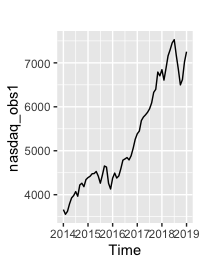
\includegraphics[width=0.43\textwidth, height=0.43\textwidth]{../assets/nasdaq.png}\label{fig:f1}}
            \subfloat[Differenced Nasdaq]{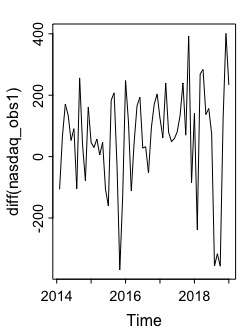
\includegraphics[width=0.4\textwidth, height=0.4\textwidth]{../assets/nasdaq_diff.png}\label{fig:f2}}
            \caption{Original v. Stationarized}
        \end{figure}
        
        It is important to note that our model has $p=0$ for AR component coefficient and $q=0$ for MA component coefficient, while having a differencing order of $1$. This means that we will be differencing the data once to make it stationary and calculate its approximate entropy to quantify randomness, to be able to compare it with white noise which serves as the foundation of ARIMA(p,d,q). When a time series data is stationary, it means the data has no significant change in mean or variance. Figure 1.a shows Nasdaq price vs time, and Figure 1.b shows the differentiated Nasdaq price over time, in other words a plot of periodic returns.
        
        \begin{figure}[htbp]
            \centering
            \subfloat[]{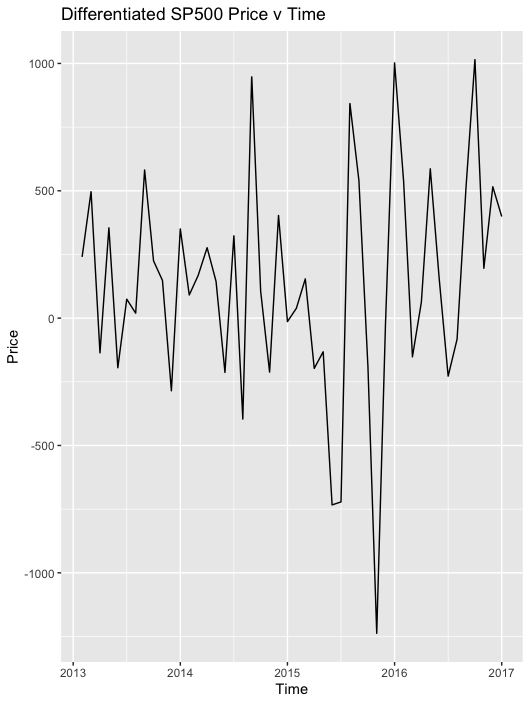
\includegraphics[width=0.48\textwidth]{../assets/diff_sp500.png}}
            \hfill
            \subfloat[]{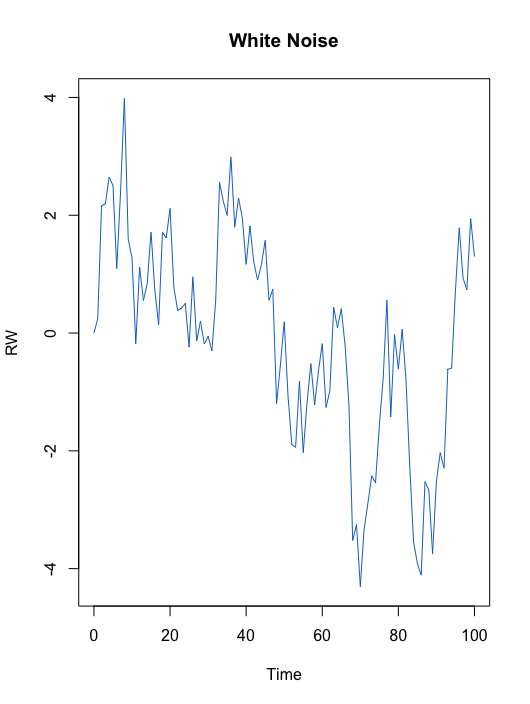
\includegraphics[width=0.52\textwidth]{../assets/whitenoise.png}}
            \caption{Differentiated Data v. White Noise}
          \end{figure}

          The resemblence in movement of white nosie vs differentiated price data can be observed in Figure 2. Many academics have also reached consensus on the success of white noise in modeling price data when seasonality and trend are stripped of the data, which is the reason why log difference is taken.[2]

        \subsection{One Way ANOVA}
        Analysis of Variance (ANOVA) is a statistical technique that is used to determine whether there is a significant difference between the means of two or more groups. The ANOVA test is used when there are multiple groups, and we want to compare the means of each group to determine whether there is a significant difference between them. The ANOVA test is based on the assumption that the data is normally distributed and that the variances of the different groups are equal.

        The basic idea behind ANOVA is to compare the variation between groups to the variation within groups. If the variation between groups is much greater than the variation within groups, then there is a significant difference between the groups, and we can reject the null hypothesis. The null hypothesis for ANOVA is that there is no significant difference between the means of the groups, and the alternative hypothesis is that there is a significant difference between the means of the groups. The test is based on the F-statistic, which is the ratio of the variation between groups to the variation within groups. If the F-statistic is large, then there is a significant difference between the means of the groups, and we can reject the null hypothesis.
        
        There are different types of ANOVA tests depending on the number of groups being compared and the type of experimental design. We will be using a One-way ANOVA when there is only one independent variable, and it has more than two levels. The single independent variable is Equity indexes and the levels are different combination of stocks forming different equities
    
        
    \section{Experiment Design}

        \textbf{Sampling Unit} 
        This study sample consisted of three different stocks as multiple levels of a single factor ANOVA design. These stocks are all featured by the huge market cap between \$10 billion and \$200 billion and their shares mostly belong to the public. In other words, the stock prices are less likely to be manipulated by nonsignificant factors and the asset is less volatile since the market is well established and therefore the data is more reliable.

        \textbf{Equipment}
        As the intention of our study is to test the validity of ARIMA model, we utilized 5 years of dependable data for input from Kaggle. Since we are dealing with time series data and model adequacy, we used \codeword{library(tseries)} to process time series data and \codeword{library(ggplot)} to visualize White Noise. In order to calculate the approximate entropy of time series data, we used \codeword{library(TSEntropies)}. The experiment will use Analysis of Variance, where observations (time intervals) will be used as blocks to mitigate the differences of approximate entropy due to times of volatility. Time intervals will be of same length, chosen at random.

        \medskip
            \begin{center}
                \begin{tabular}{ |p{2cm}||p{2cm}|p{2cm}|p{2cm}|p{2cm}|}
                    \hline
                    \multicolumn{5}{|c|}{Stock | Observations} \\
                    \hline
                    Equity Index&$t_{1}$      &$t_{2}$    &$t_{3}$    &$t_{4}$    \\
                    \hline
                    NASDAQ      &$y_{1,1}$   &$y_{1,2}$  &$y_{1,3}$  &$y_{1,4}$  \\
                    SP500       &$y_{2,1}$   &$y_{2,2}$  &$y_{2,3}$  &$y_{2,4}$  \\
                    DOWJU       &$y_{3,1}$   &$y_{3,2}$  &$y_{3,3}$  &$y_{3,4}$  \\
                    DOWJT       &$y_{3,1}$   &$y_{3,2}$  &$y_{3,3}$  &$y_{4,4}$  \\
                    \hline
                \end{tabular}
                \captionof{table}{Observations Table} 
        \end{center}

            \begin{hyp}{0} 
                Observed index stocks are of same irregularity, one market is not significantly more random than the others.
                $\mu_{1}$ = $\mu_{2}$ = $\mu_{3}$ \dots $\mu_{n}$  
            \end{hyp}
            \begin{hyp}{1} 
                Observed index stock prices are not of same irregularity, at least one market is significantly more random than the others.
                $\mu_{a} \neq \mu_{b}$ where \( \mu_{a},\mu_{b} \in \{\mu_{1}, \mu_{2},\mu_{3}, \dots, \mu_{n} \} \)
            \end{hyp}
            \medskip

            \textbf{Dependent Variable} of this experiment is the approximate entropy of the log differentiated price for each market.
            \medskip

            \textbf{Independent Variable} of this experiment are stock prices, with 4 different levels included to represent different industries.

        \section{Data Processing}
            \subsection{Preprocessing}
                \textbf{Granularity} 10 years monthly price data fetched from Fred for S\&P500 companies and loaded into R workstation. To address known performance issues of ARIMA, daily data was converted into monthly price average data with a frequency of 12 from FRED's Graphical User Interface.

                \textbf{Stationary Data} ARIMA(0,0,0) works best on data with no trend and constant variance. Most financial instruments, including stock prices have a trend with non-constant variance. In order to prepare the data for ARIMA timeseries forecast, we will compute the difference of logs for each data set and conduct a Dick \& Fuller's (DF) test. The  results of the function \codeword{adf.test(data)} from \codeword{library(tseries)} on the differenced timeseries data \codeword{diff(ts_obs1)}, will yield a p-value where 
                \begin{hyp}{0} 
                    $p>0.05$, Time series data is not stationary.
                \end{hyp}
                \begin{hyp}{1} 
                    $p<0.05$, Time series data is stationary
                \end{hyp}
                meaning time series with a DF result of $p<0.05$ are workable with ARIMA. For time series that failed DF test the first differentiation will be differenced again.

                \textbf{Date} Date format should be converted to MM-DD-YY in order to create a timeseries object R can work with.

            \subsection{Data Collection}
                In order to test the generalization of white noise modeling, we will be testing index prices of securities from different industries. We will be looking at SP500, NASDAQ, DJIA, DJTA 
                
                A quantitative difference regarding securities of different industries is the change in volatility and trend strength. This apparent difference in volatility among indexes was not chosen by the experimenters, but rather a natural result due to the change in risk appetites of the investors of corresponding industries. Trend and seasonality is expected to be mitigated using logarithm and differentiation.

        \section{Results}
                The recorded entropy for each index at each time window can be seen in Figure 3.a and the statistical summary for the entropy table can be seen in Figure 3.b. We can see that SP had a larger mean entropy than the rest of the markets, followed by Nasdaq.

                \begin{figure}[htbp]
                    \centering
                    \subfloat[Entropy table]{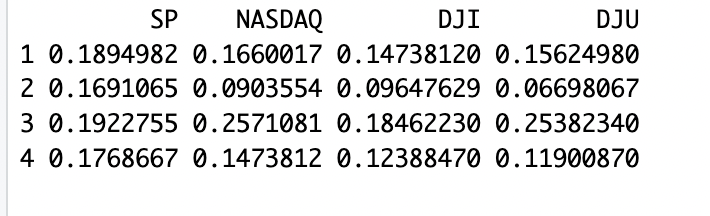
\includegraphics[width=0.48\textwidth]{../assets/entropy_table.png}}
                    \hfill
                    \subfloat[Table summary]{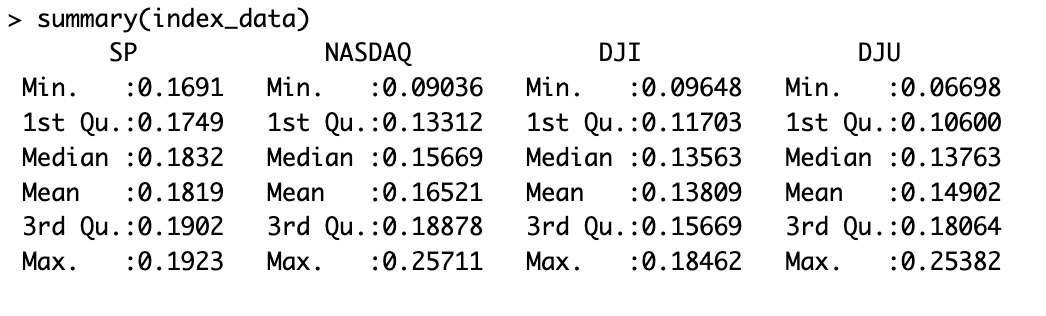
\includegraphics[width=0.52\textwidth]{../assets/entropy_summary.png}}
                    \caption{}
                  \end{figure}

                The table acquired by adjoining the entropy values of different indexes as columns are then converted into LONG form to conduct ANOVA using \codeword{melt} function from \codeword{reshape2} package. The resulting ANOVA results can be seen in Table 2:

                  \begin{center}
                    \begin{tabular}{ |p{2cm}|p{1cm}|p{2cm}|p{2cm}|p{2cm}|p{2cm}|}
                        \hline
                                   & Df &Sum Sq  &Mean Sq  &F Value &Pr( $>$F)\\
                        \hline
                        Markets    &3   &0.00440 &0.00147  &0.469   &0.710  \\
                        Residuals  &12  &0.0376  &0.00313  &        &  \\
                        Total      &15  &0.042  &  &        &  \\
                        \hline
                    \end{tabular}
                    \captionof{table}{ANOVA Table} 
                \end{center}

                    It's important to note in Figure 3.a, the range of values pertaining to row 3 have a significantly larger mean of entropy. Row 3 data refers to price data that was collected between 2015 - 2020 for 4 different indexes. The prices collected during this time window were largely affected by the selling pressure due to COVID virus. The following Figure shows the original prices plotted against time:

                    \begin{figure}[htbp]
                      \centering
                      \subfloat[NASDAQ]{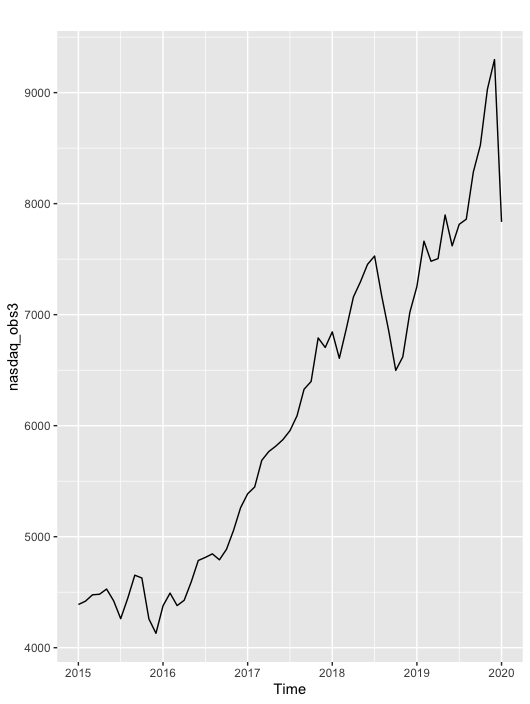
\includegraphics[width=0.5\textwidth]{../assets/nasdaq_covid.png}}
                      \hfill
                      \subfloat[SP500]{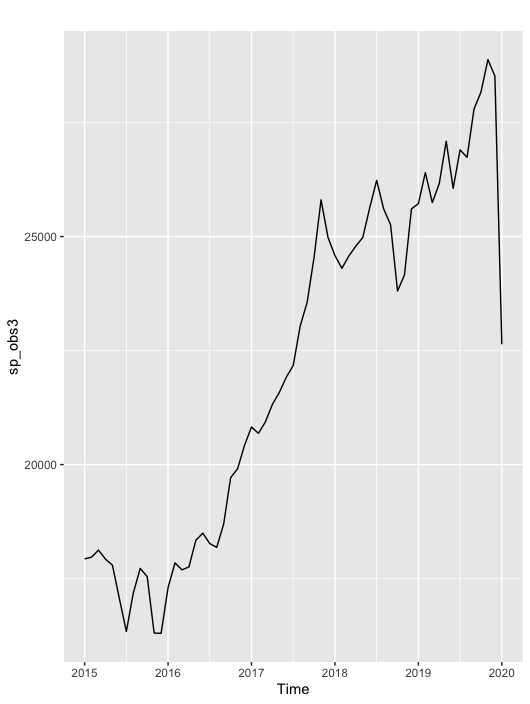
\includegraphics[width=0.5\textwidth]{../assets/sp_covid.png}}
                      \caption{}
                    \end{figure}

                    The sharp drop due to COVID sell-off can be better seen when the time series is differentiated once. The experimenters did not remove the aforementioned unhealthy results to keep the sampling process random. See Figure 5 for the log differentiated, \codeword{diff(log(sp_obs1))} price plots.

                    \begin{figure}[htbp]
                        \centering
                        \subfloat[Differentiated NASDAQ]{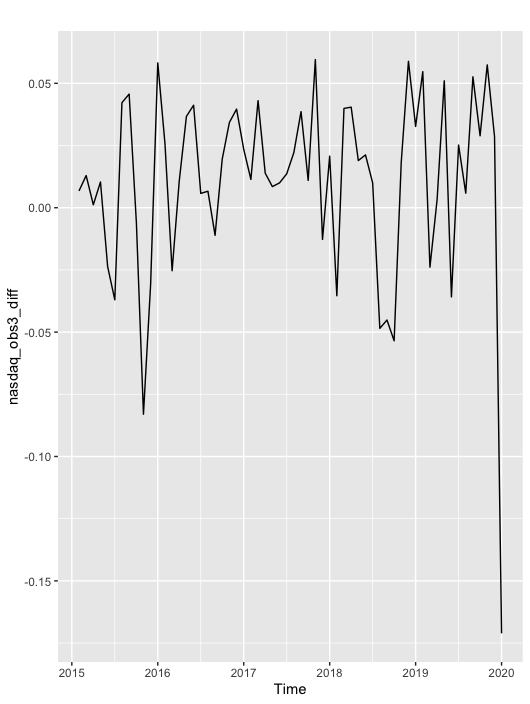
\includegraphics[width=0.45\textwidth, height=0.3\textwidth]{../assets/nasdaq_covid_digg.png}}
                        \hfill
                        \subfloat[Differentiated SP500]{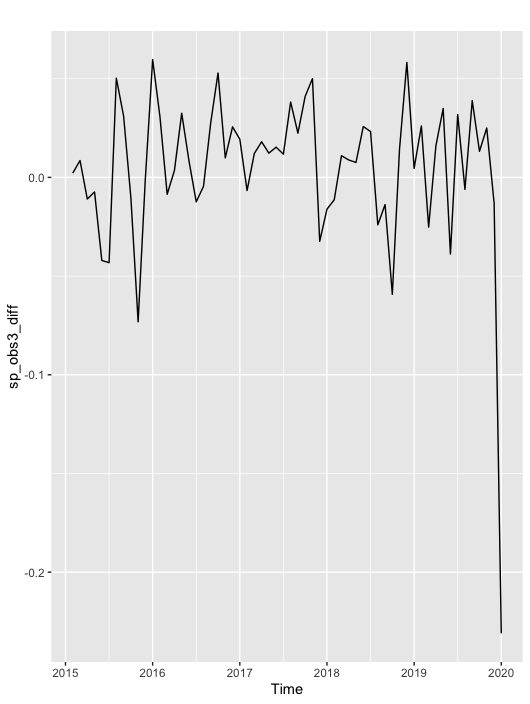
\includegraphics[width=0.45\textwidth, height=0.3\textwidth]{../assets/sp_covid_diff.png}}
                        \caption{}
                      \end{figure}

                  We analyzed 4 different levels, which resulted in 3 degrees of freedom for markets and 12 degrees of freedom for residuals given we had 4 observations. From the F Table in Appendix \ref{appendix:f_table}, we observed the critical Value for F with the following parameters, Df1 = 3, Df2 = 12, $\alpha = 0.05$ which yields: 
                  \[F_{c} = F_{0.05,3,12} = 3.49 \]
                    since \(F < F_c \), we conclude there are no significant difference between markets in terms of entropy. 

                  \begin{figure}[htbp]
                    \centering
                    \subfloat[Q-Q Plot]{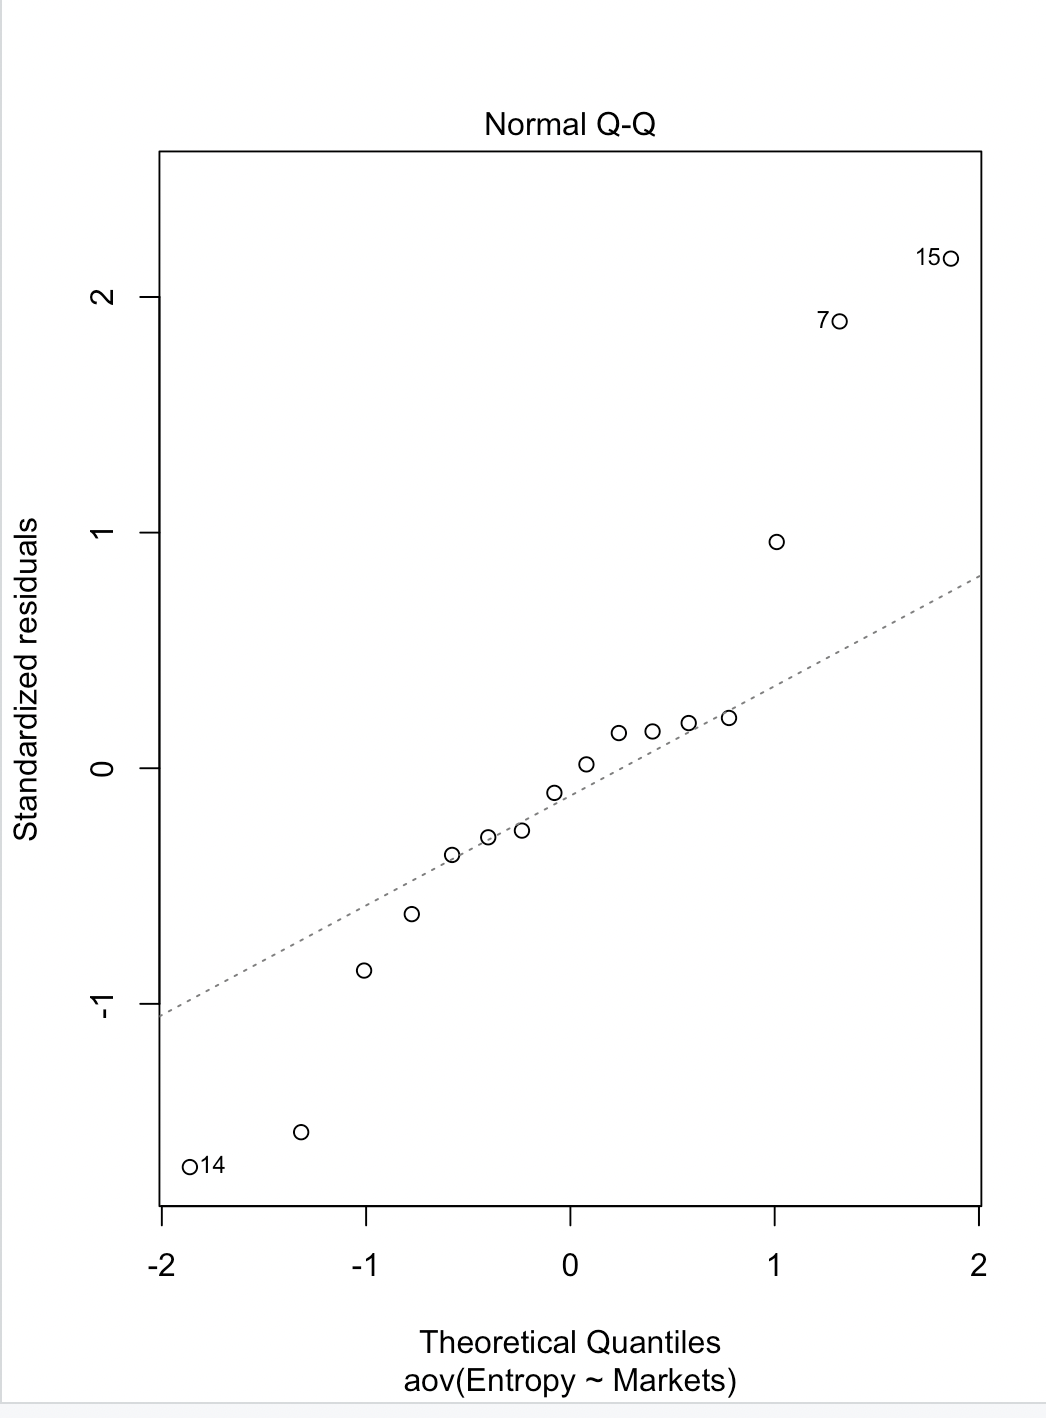
\includegraphics[width=0.5\textwidth]{../assets/qq.png}}                    
                    \hfill
                    \subfloat[Residual v Fitted]{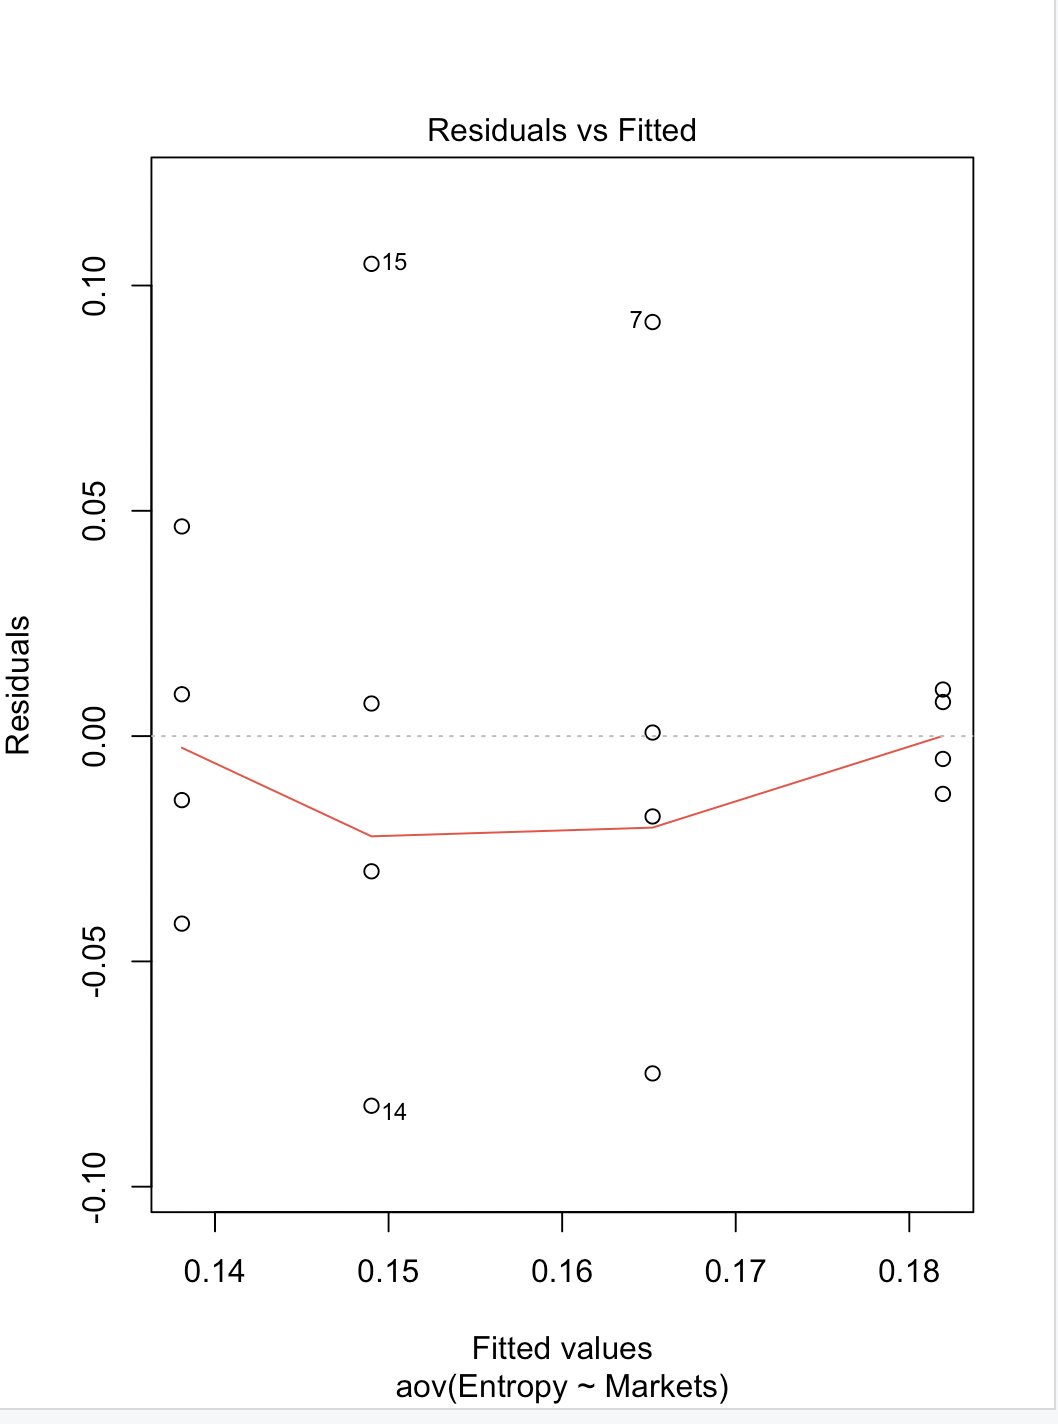
\includegraphics[width=0.5\textwidth]{../assets/residual_fitted.png}}
                    \caption{Adequacy Checking}
                  \end{figure}

                  \textbf{QQ Plot} The points follow the line closely, we can assume the data is normally distributed.

                  \textbf{Residual v Fitted} The points appear to be random, with no apparent trend. There is a slight curve seen in the middle of the plot, but the evidence isn't enought to conclude non-normal distribution for this experiment.

        \section{Discussion}
            \subsection{Evaluation}
                We have recorded the entropy values for NASDAQ, SP500, DOWJIA and DOWJTA markets observed for 5 years, replicated for four times. We have stationarized the log scaled data to calculate and compare the approximate entropy for each stock, of each time window. We have conducted Analysis of Variance for this data to compare the variance between different markets to the variance within; in order to make a conclusion about whether entropy changes from market to market. 
                

            \subsection{Limitations \& Future Work}
                As is the case for most experiments, we expect to see more accurate results with a replication on a higher scale.

                \textbf{Observations} Due to time constraints of course schedule, we were only able to conduct the experiment for 4 different time windows. In order to observe the appearance of Random Walk, we need to collect more observations to make sure the hypothesized independent and identically distributed behavior of markets converge. Even though one way anova has a minimum required numer of observations of 3, estimating the randomness inherently requires a large number of observations conducted on a large numer of IV levels.

                \textbf{Levels} Also the number of levels of independent variable, equity indexes, were limited to four - which in return increases the room for error. If we had included more levels of our independent variable,
                
                \textbf{Overlap} As much as we tried to pick indexes so that they have small overlap in terms of stocks included, the prominent indexes such as SP500 include a wide range of popular assets, which are also chosen by other indexes. This small but direct correlation between levels of independent variable hinders the accuracy of the experiment.

            \section{Conclusion}
                In this paper, we have conducted ANOVA on the observations of entropy calculations for 4 different equity indexes; repeated the observation for randomly selected time windows out of the available data for four different times. We aimed to find out if the entropy for each equity index is the same across different industries. The ticker with higher entropy would resemble white noise returns or random walk price movement.

                According to our ANOVA results, we couldn't find signficant entropy difference between the aforementioned markets, with respect to 5-yr time windows chosen. The findings are parallel to the theoru of modeling financial markets with Random Walk or modeling stock market returns with white noise. We conclude that there is no significant evidence to prove the set of markets: NASDAQ, SP500, DOWJIA, DOWJTA have an outlier in terms of approximate entropy or irregularity.

                
            \begin{thebibliography}{2}
                \bibitem{texbook}
                Pincus S, Kalman RE. Irregularity, volatility, risk, and financial market time series. Proc Natl Acad Sci U S A. 2004 Sep 21;101(38):13709-14. doi: 10.1073/pnas.0405168101. Epub 2004 Sep 9. PMID: 15358860; PMCID: PMC518821.

                \bibitem{texbook}
                Pincus, S. M. Approximate entropy as a measure of system complexity. Proceedings of the National Academy of Sciences 88, 22972301 (1991).

            \end{thebibliography}


            \begin{appendices}
                \section{F Table}
                \label{appendix:f_table}
                \begin{figure}[htbp]
                    \subfloat[F Table]{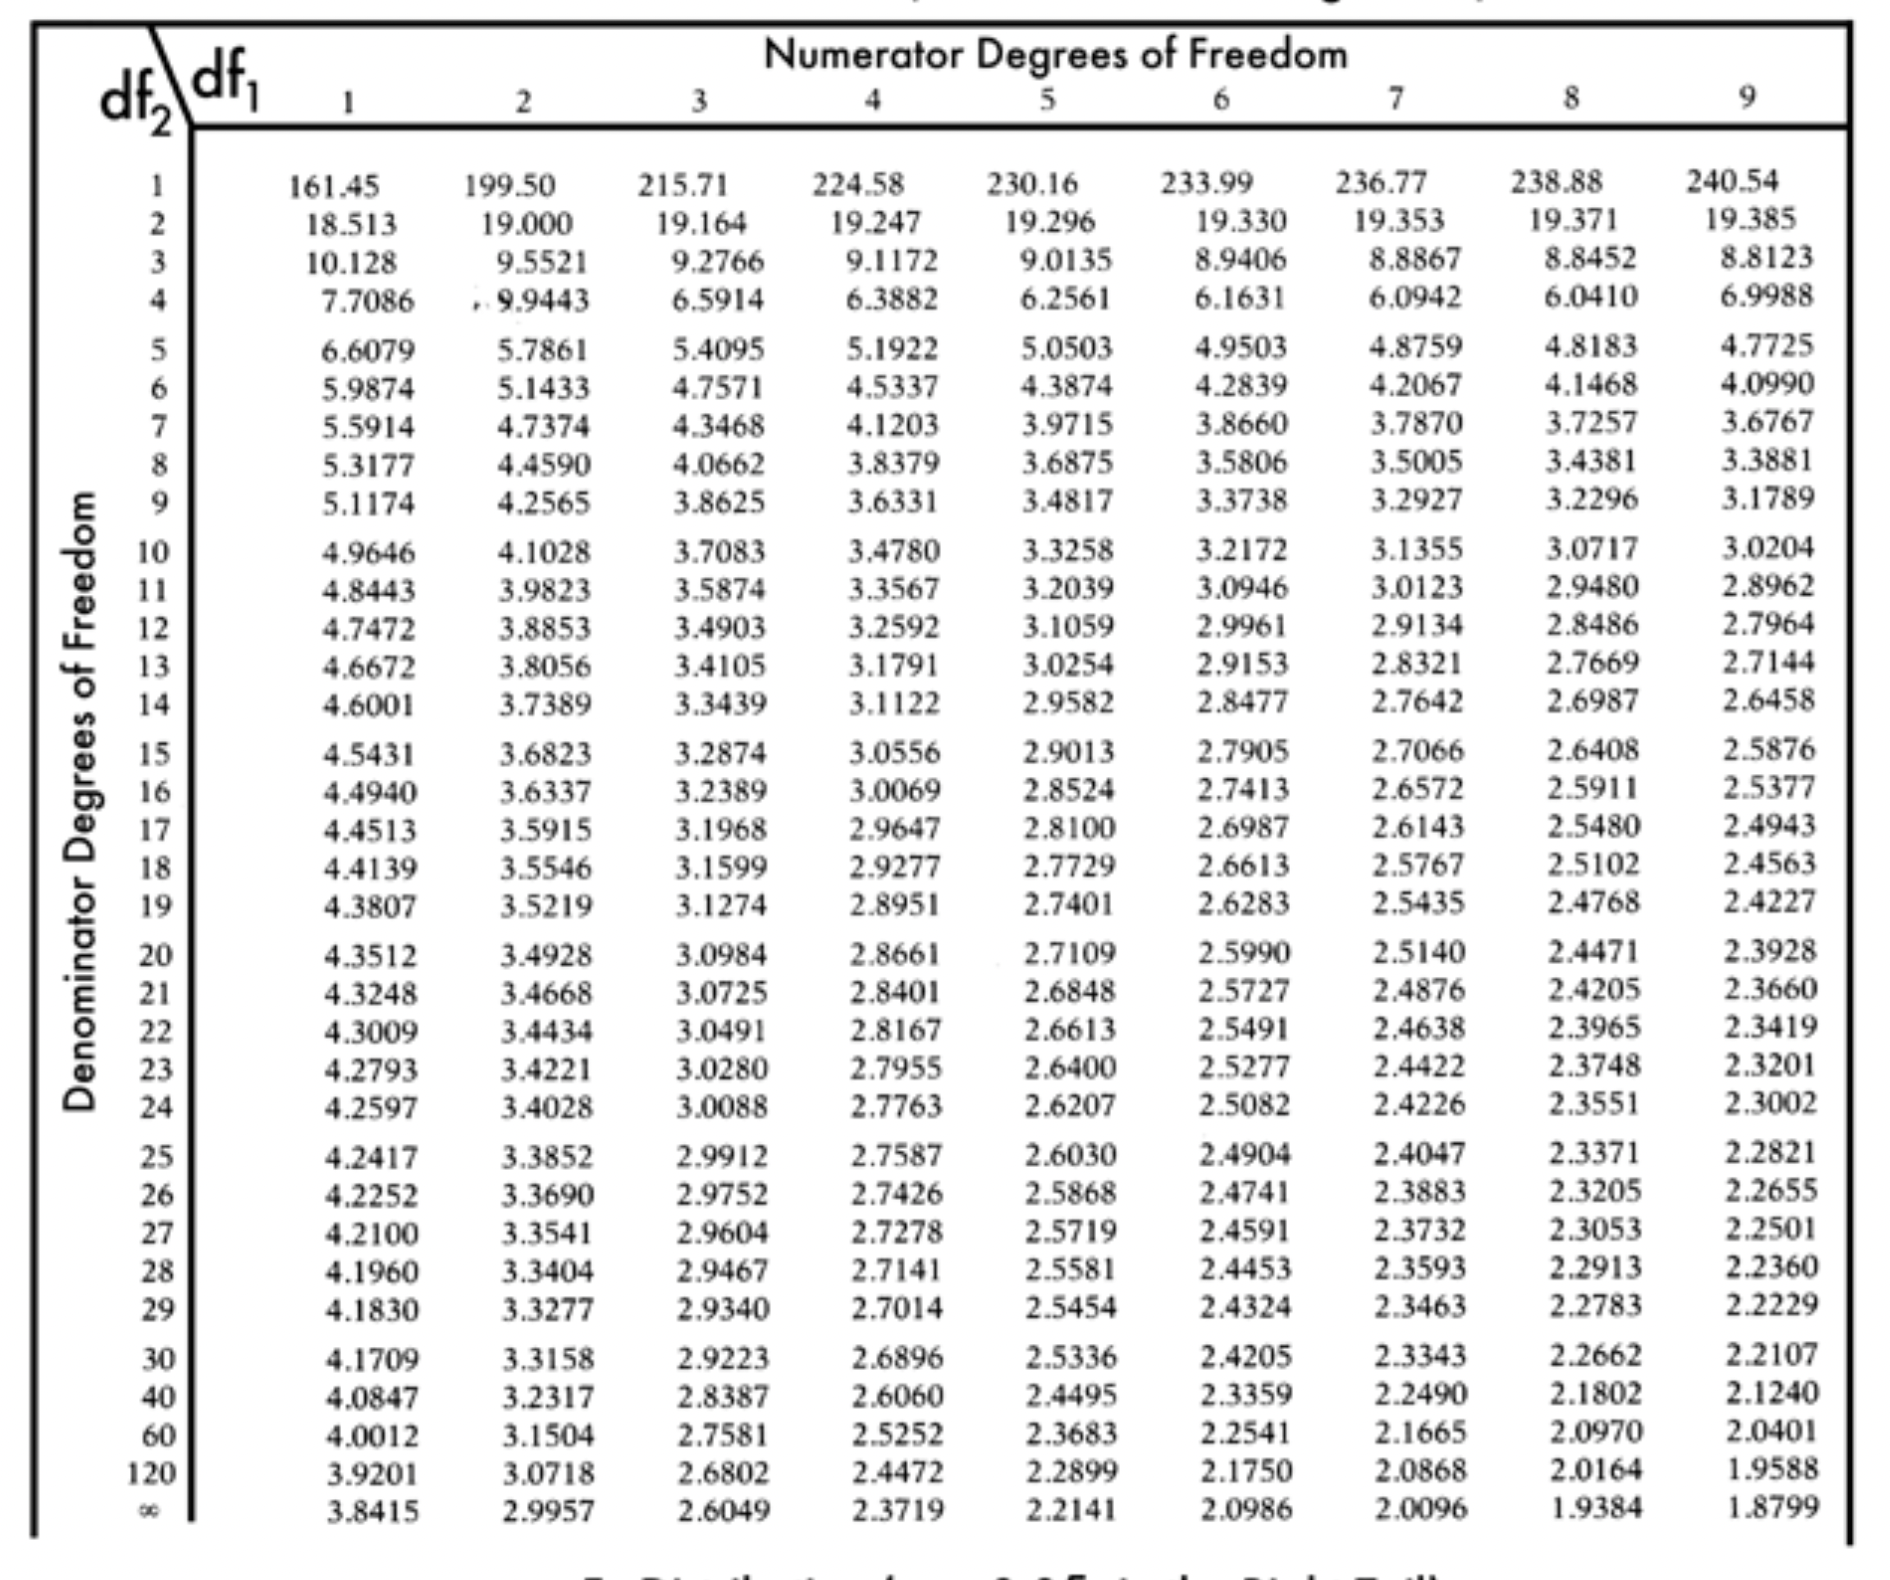
\includegraphics[width=0.8\textwidth]{../assets/appendix1.png}}                    
                    \end{figure}    

                \section{R Script}
                \begin{lstlisting}
library(forecast)
library(ggplot2)
library(tseries)
library(TSEntropies)
library(reshape2)
setwd("/Users/orhankoc/Documents/ARIMA_RCBD/scipts")


RW <- arima.sim(model= list(order = c(0, 0, 0)), n=60)
plot.ts(RW,main="White Noise", col=4)
autoplot(diff(sp_obs2)) + labs( y="Price", title="Differentiated SP500 Price v Time")

################################################################################
#                                   ARIMA                                      #
################################################################################
# independent variable 1: SP500, monthly data                                  #
#______________________________________________________________________________#
# https://fred.stlouisfed.org/series/SP500#0
SP = read.csv("SP500.csv")
SP_ts <- ts(SP$DJIA, start=c(2013, 1), end=c(2022, 3), frequency=12)
# minimum sample is n=50 recommended for ARIMA
sp_obs1 <- window(SP_ts, c(2014), c(2019, 1))
sp_obs2 <- window(SP_ts, c(2012), c(2017, 1))
sp_obs3 <- window(SP_ts, c(2015), c(2020, 1))
sp_obs4 <- window(SP_ts, c(2013), c(2018, 1))

# Step 2: Check for stationarity
autoplot(sp_obs1)
autoplot(sp_obs2)  
autoplot(sp_obs3)   
autoplot(sp_obs4)  

sp_obs1_diff <- diff(log(sp_obs1))
sp_obs2_diff <- diff(log(sp_obs2))
sp_obs3_diff <- diff(log(sp_obs3))
sp_obs4_diff <- diff(log(sp_obs4))

autoplot(sp_obs1_diff) 
autoplot(sp_obs2_diff) 
autoplot(sp_obs3_diff) 
autoplot(sp_obs4_diff) 

# check if difference of log data is stationary for SP500 using Dick Fulley test
#H0: The time series is non-stationary.
#HA: The time series is stationary.
adf.test(sp_obs1_diff) # is stationary
adf.test(sp_obs2_diff) # is NOT stationary
adf.test(sp_obs3_diff) # is NOT stationary
adf.test(sp_obs4_diff) # is stationary

# APPROXIMATE ENTROPY:
ApEn(RW, r = 0.1*sd(RW))
ApEn(sp_obs1_diff, r = 0.1*sd(sp_obs1_diff)) # 0.1894982
ApEn(sp_obs2_diff, r = 0.1*sd(sp_obs2_diff)) # 0.1691065
ApEn(sp_obs3_diff, r = 0.1*sd(sp_obs3_diff)) # 0.1922755
ApEn(sp_obs4_diff, r = 0.1*sd(sp_obs4_diff)) # 0.1768667

################################################################################
# independent variable 2: NASDAQ, monthly data                                 #
#______________________________________________________________________________#
# https://fred.stlouisfed.org/series/NASDAQ100#0
NASDAQ = read.csv("NASDAQ100.csv")
nasdaq_ts <- ts(NASDAQ$NASDAQ100, start=c(2013,1), end=c(2022, 3), frequency=12)

nasdaq_obs1 <- window(nasdaq_ts, c(2014), c(2019, 1))
nasdaq_obs2 <- window(nasdaq_ts, c(2012), c(2017, 1))
nasdaq_obs3 <- window(nasdaq_ts, c(2015), c(2020, 1))
nasdaq_obs4 <- window(nasdaq_ts, c(2013), c(2018, 1))

# Step 2: Check for stationarity
autoplot(nasdaq_obs1)
autoplot(nasdaq_obs2)
autoplot(nasdaq_obs3)
autoplot(nasdaq_obs4)

nasdaq_obs1_diff <- diff(log(nasdaq_obs1))
nasdaq_obs2_diff <- diff(log(nasdaq_obs2))
nasdaq_obs3_diff <- diff(log(nasdaq_obs3))
nasdaq_obs4_diff <- diff(log(nasdaq_obs4))

autoplot(nasdaq_obs1_diff)
autoplot(nasdaq_obs2_diff)
autoplot(nasdaq_obs3_diff)
autoplot(nasdaq_obs4_diff)

# check if difference of log data is stationary for SP500 using Dick Fulley test
#H0: The time series is non-stationary.
#HA: The time series is stationary.
adf.test(nasdaq_obs1_diff) # is stationary
adf.test(nasdaq_obs2_diff) # is NOT stationary
adf.test(nasdaq_obs3_diff) # is stationary
adf.test(nasdaq_obs4_diff) # is stationary

ApEn(nasdaq_obs1_diff, r = 0.1*sd(nasdaq_obs1_diff)) # 0.1660017
ApEn(nasdaq_obs2_diff, r = 0.1*sd(nasdaq_obs2_diff)) # 0.0903554
ApEn(nasdaq_obs3_diff, r = 0.1*sd(nasdaq_obs3_diff)) # 0.2571081
ApEn(nasdaq_obs4_diff, r = 0.1*sd(nasdaq_obs4_diff)) # 0.1473812

################################################################################
# independent variable 3: DOWJ Transportation average, monthly data            #
#______________________________________________________________________________#
# https://fred.stlouisfed.org/series/DJTA#0
DJT = read.csv("DJTA.csv")

DJT_ts <- ts(DJT$DJTA, start=c(2013,1), end=c(2022, 3), frequency=12)
djt_obs1 <- window(DJT_ts, c(2014), c(2019, 1))
djt_obs2 <- window(DJT_ts, c(2012), c(2017, 1))
djt_obs3 <- window(DJT_ts, c(2015), c(2020, 1))
djt_obs4 <- window(DJT_ts, c(2013), c(2018, 1))

# Step 2: Check for stationarity
autoplot(djt_obs1)
autoplot(djt_obs2)
autoplot(djt_obs3)
autoplot(djt_obs4)

djt_obs1_diff <- diff(log(djt_obs1))
djt_obs2_diff <- diff(log(djt_obs2))
djt_obs3_diff <- diff(log(djt_obs3))
djt_obs4_diff <- diff(log(djt_obs4))

autoplot(djt_obs1_diff)
autoplot(djt_obs2_diff)
autoplot(djt_obs3_diff)
autoplot(djt_obs4_diff)

# check if difference of log data is stationary for SP500 using Dick Fulley test
#H0: The time series is non-stationary.
#HA: The time series is stationary.
adf.test(djt_obs1_diff) # is stationary
adf.test(djt_obs2_diff) # is NOT stationary
adf.test(djt_obs3_diff) # is stationary
adf.test(djt_obs4_diff) # is NOT stationary

ApEn(djt_obs1_diff, r = 0.1*sd(djt_obs1_diff)) # 0.1473812
ApEn(djt_obs2_diff, r = 0.1*sd(djt_obs2_diff)) # 0.09647629
ApEn(djt_obs3_diff, r = 0.1*sd(djt_obs3_diff)) # 0.1846223
ApEn(djt_obs4_diff, r = 0.1*sd(djt_obs4_diff)) # 0.1238847

################################################################################
# independent variable 4: DOWJ Utility average, monthly data                   #
#______________________________________________________________________________#
# https://fred.stlouisfed.org/series/DJUA#0
DJU= read.csv("DJUA.csv")

DJU_ts <- ts(DJU$DJUA, start=c(2013,1), end=c(2022, 3), frequency=12)
dju_obs1 <- window(DJU_ts, c(2014), c(2019, 1))
dju_obs2 <- window(DJU_ts, c(2012), c(2017, 1))
dju_obs3 <- window(DJU_ts, c(2015), c(2020, 1))
dju_obs4 <- window(DJU_ts, c(2013), c(2018, 1))

# Step 2: Check for stationarity
autoplot(dju_obs1)
autoplot(dju_obs2)
autoplot(dju_obs3)
autoplot(dju_obs4)

dju_obs1_diff <- diff(log(dju_obs1))
dju_obs2_diff <- diff(log(dju_obs2))
dju_obs3_diff <- diff(log(dju_obs3))
dju_obs4_diff <- diff(log(dju_obs4))

autoplot(dju_obs1_diff)
autoplot(dju_obs2_diff)
autoplot(dju_obs3_diff)
autoplot(dju_obs4_diff)

# check if difference of log data is stationary for SP500 using Dick Fulley test
#H0: The time series is non-stationary.
#HA: The time series is stationary.
adf.test(dju_obs1_diff) # p<0.05, Reject H0 at d=1, is stationary
adf.test(dju_obs2_diff) # p>0.05, Reject H0 at d=1, NOT stationary
adf.test(dju_obs3_diff) # p<0.05, Reject H0 at d=1, NOT stationary
adf.test(dju_obs4_diff) # p<0.05, Reject H0 at d=1, is stationary

ApEn(dju_obs1_diff, r = 0.1*sd(dju_obs1_diff)) # 0.1562498
ApEn(dju_obs2_diff, r = 0.1*sd(dju_obs2_diff)) # 0.06698067
ApEn(dju_obs3_diff, r = 0.1*sd(dju_obs3_diff)) # 0.2538234
ApEn(dju_obs4_diff, r = 0.1*sd(dju_obs4_diff)) # 0.1190087
################################################################################
#                               ONE WAY ANOVA                                  #
################################################################################

# ENTROPY ANOVA
SP = c(0.1894982, 0.1691065, 0.1922755, 0.1768667)
NASDAQ = c(0.1660017, 0.0903554, 0.2571081, 0.1473812)
DJI = c(0.1473812, 0.09647629, 0.1846223, 0.1238847)
DJU = c(0.1562498, 0.06698067, 0.2538234, 0.1190087)

index_data = data.frame(SP, NASDAQ, DJI, DJU)
index_data

colnames(index_data)
index_data$id <- c(1,2,3,4,5,6,7,8,9,10,11,12,13,14,15,16)
index_data$id

index_data$Markets

summary(index_data)

index_data_long <- melt(index_data, 
                    variable.name = "Markets", 
                    value.name = "Entropy") 

model = aov(Entropy ~ Markets, index_data_long)
summary(model)
plot(model)




                        \end{lstlisting}
                    
            \end{appendices}

\end{document}